% !Mode:: "TeX:UTF-8"
% !TeX encoding = UTF-8 Unicode
% !TeX program = xelatex

%%%%%%%%%%%%%%%%%%%%%%%%%%%%%%%%%%%%%%%%%%%%%%%%%%%%%%%%%%%%%%%%%%%
% overleaf 中会报警告Package fontspec Warning: 
% Font "FandolSong-Regular""FandolHei-Regular""FandolFang-Regular" 
% does not contain requested Script "CJK".
% xeLatex本身的问题,下面这句强制静音这个警告,本地环境下可以注释
\PassOptionsToPackage{quiet}{fontspec}
%%%%%%%%%%%%%%%%%%%%%%%%%%%%%%%%%%%%%%%%%%%%%%%%%%%%%%%%%%%%%%%%%%%

\documentclass[master]{jnthesis}       % doctor*, master, nodegree 【本地环境用这个】
	% !Mode:: "TeX:UTF-8"
% !TeX encoding = UTF-8 Unicode
% !TeX program = xelatex
% !TeX root = ../root.tex

%%%%%%%%%%%%%%%%%%%%%%%%%%%%%%%%%%%%%%%%%%
%%%             用户设置               %%%
%%%%%%%%%%%%%%%%%%%%%%%%%%%%%%%%%%%%%%%%%%
%%%%%%%%%%%%%%%%%%%%%%%%%%%%%%%%%%%%%%%%%%
%%% 题目, 作者, 日期 (用于标题页)
\title{论文题目}
\author{作者}
\date{\today}
%%%%%%%%%%%%%%%%%%%%%%%%%%%%%%%%%%%%%%%%%%


%%%%%%%%%%%%%%%%%%%%%%%%%%%%%%%%%%%%%%%%%%
%%% 设置插图文件路径
\graphicspath{{figures/}} % 插图文件路径 (以 / 结尾)
%%%%%%%%%%%%%%%%%%%%%%%%%%%%%%%%%%%%%%%%%%

%%%%%%%%%%%%%%%%%%%%%%%%%%%%%%%%%%%%%%%%%%
%%% 修改中英文字体
% CTEX默认正文宋体,注释下面这句
% \setCJKmainfont[AutoFakeBold={2.17}]{SimSun}
\setmainfont{Times New Roman}
%%%%%%%%%%%%%%%%%%%%%%%%%%%%%%%%%%%%%%%%%%

%%%%%%%%%%%%%%%%%%%%%%%%%%%%%%%%%%%%%%%%%%
%%% 其他宏包
\usepackage{tikz}             % Tikz 绘图
\usepackage{pgfplots}         % PGFPlots 图表
\pgfplotsset{compat=newest}
\usepgfplotslibrary{external} % 生成图表文件
\tikzexternalize              % 生成图文件

%%%%%%%%%%%%%%%%%%%%%%%%%%%%%%%%%%%%%%%%%%

%%%%%%%%%%%%%%%%%%%%%%%%%%%%%%%%%%%%%%%%%%
%%% 其他设置

% 会报警告
\setlength{\headheight}{27pt}

% mathrsfs这个宏包报警告 Font shape `U/rsfs/m/n' in size <15.05624> not available
\DeclareFontFamily{U}{rsfs}{\skewchar\font127 }
\DeclareFontShape{U}{rsfs}{m}{n}{%
   <-6.5> rsfs5
   <6.5-8> rsfs7
   <8-> rsfs10
}{}

%%%%%%%%%%%%%%%%%%%%%%%%%%%%%%%%%%%%%%%%%%
% 链接样式
\hypersetup{
  colorlinks=true,
  linkcolor=black,
  citecolor=black,
}

%%%%%%%%%%%%%%%%%%%%%%%%%%%%%%%%%%%%%%%%%%
% 公式编号 (c.s.n)
%\renewcommand{\theequation}{\arabic{chapter}.\arabic{section}.\arabic{equation}}


%%%%%%%%%%%%%%%%%%%%%%%%%%%%%%%%%%%%%%%%%%
%\usepackage{syntonly} % 快速检查错误, 分页但不生成 DVI 输出结果
%\syntaxonly           % 仅检查语法, 不分页(更快速)

%\includeonly{body/ch01}
%\includeonly{body/ch02}
%\includeonly{body/ch03}
%\includeonly{body/ch04}
%\includeonly{body/ch05}
%\includeonly{body/ch06}
%\includeonly{body/ch07}

%%%%%%%%%%%%%%%%%%%%%%%%%%%%%%%%%%%%%%%%%%
             % 用户设置
	% !Mode:: "TeX:UTF-8"
% !TeX encoding = UTF-8 Unicode
% !TeX program = xelatex
% !TeX root = ../root.tex

%% 自定义符号

% 集合
\providecommand{\bbN}{{\mathbb N}} % 自然数
\providecommand{\bbZ}{{\mathbb Z}} % 整数
\providecommand{\bbR}{{\mathbb R}} % 实数
\providecommand{\bbC}{{\mathbb C}} % 复数
\providecommand{\bbF}{{\mathbb F}} % 数域(实数或复数)

\providecommand{\nn}{{n \times n}} % n x n
\providecommand{\bbRn}{{\mathbb{R}^n}} % R^n
\providecommand{\bbRnn}{{\mathbb{R}^{n \times n}}} % R^(nxn)

% 转置
\providecommand{\rmT}{{\mathrm{T}}}
% diag
\providecommand{\diag}{{\operatorname{diag}}}
% tr
\providecommand{\tr}{{\operatorname{tr}}}

% 积分和导数
\providecommand{\dx}{{{\,\mathrm{d}}x}}
\providecommand{\dy}{{{\,\mathrm{d}}y}}
\providecommand{\dz}{{{\,\mathrm{d}}z}}
\providecommand{\dt}{{{\,\mathrm{d}}t}}
\providecommand{\ds}{{{\,\mathrm{d}}s}}
\providecommand{\dtau}{{{\,\mathrm{d}}\tau}}
\providecommand{\ddx}{\frac{\mathrm{d}}{{\mathrm{d}}x}}
\providecommand{\ddy}{\frac{\mathrm{d}}{{\mathrm{d}}y}}
\providecommand{\ddz}{\frac{\mathrm{d}}{{\mathrm{d}}z}}
\providecommand{\ddt}{\frac{\mathrm{d}}{{\mathrm{d}}t}}
\providecommand{\dds}{\frac{\mathrm{d}}{{\mathrm{d}}s}}
\providecommand{\ddtau}{\frac{\mathrm{d}}{{\mathrm{d}}\tau}}

% 希腊字母
\providecommand{\xa}{\alpha}
\providecommand{\xb}{\beta}
\providecommand{\xch}{\chi}
\providecommand{\xd}{\delta}
\providecommand{\xcd}{\Delta}
\providecommand{\xe}{\epsilon}
\providecommand{\xve}{\varepsilon}
\providecommand{\xet}{\eta}
\providecommand{\xg}{\gamma}
\providecommand{\xcg}{\Gamma}
\providecommand{\xio}{\iota}
\providecommand{\xl}{\lambda}
\providecommand{\xcl}{\Lambda}
\providecommand{\xm}{\mu}
\providecommand{\xn}{\nu}
\providecommand{\xo}{\omega}
\providecommand{\xco}{\Omega}
\providecommand{\xp}{\pi}
\providecommand{\xcp}{\Pi}
\providecommand{\xvp}{\varpi}
\providecommand{\xph}{\phi}
\providecommand{\xcph}{\Phi}
\providecommand{\xvph}{\varphi}
\providecommand{\xps}{\psi}
\providecommand{\xcps}{\Psi}
\providecommand{\xs}{\sigma}
\providecommand{\xcs}{\Sigma}
\providecommand{\xvs}{\varsigma}
\providecommand{\xz}{\zeta}
\providecommand{\xr}{\rho}
\providecommand{\xvr}{\varrho}
\providecommand{\xt}{\tau}
\providecommand{\xth}{\theta}
\providecommand{\xcth}{\Theta}
\providecommand{\xvth}{\vartheta}
\providecommand{\xu}{\upsilon}
\providecommand{\xcu}{\Upsilon}
\providecommand{\xx}{\xi}
\providecommand{\xcx}{\Xi}

% 粗体
\providecommand{\bs}[1]{\boldsymbol{#1}}

% \bsa~z
\providecommand{\bsa}{\bs{a}}
\providecommand{\bsb}{\bs{b}}
\providecommand{\bsc}{\bs{c}}
\providecommand{\bsd}{\bs{d}}
\providecommand{\bse}{\bs{e}}
\providecommand{\bsf}{\bs{f}}
\providecommand{\bsg}{\bs{g}}
\providecommand{\bsh}{\bs{h}}
\providecommand{\bsi}{\bs{i}}
\providecommand{\bsj}{\bs{j}}
\providecommand{\bsk}{\bs{k}}
\providecommand{\bsl}{\bs{l}}
\providecommand{\bsm}{\bs{m}}
\providecommand{\bsn}{\bs{n}}
\providecommand{\bso}{\bs{o}}
\providecommand{\bsp}{\bs{p}}
\providecommand{\bsq}{\bs{q}}
\providecommand{\bsr}{\bs{r}}
\providecommand{\bss}{\bs{s}}
\providecommand{\bst}{\bs{t}}
\providecommand{\bsu}{\bs{u}}
\providecommand{\bsv}{\bs{v}}
\providecommand{\bsw}{\bs{w}}
\providecommand{\bsx}{\bs{x}}
\providecommand{\bsy}{\bs{y}}
\providecommand{\bsz}{\bs{z}}

% \bsA~Z
\providecommand{\bsA}{\bs{A}}
\providecommand{\bsB}{\bs{B}}
\providecommand{\bsC}{\bs{C}}
\providecommand{\bsD}{\bs{D}}
\providecommand{\bsE}{\bs{E}}
\providecommand{\bsF}{\bs{F}}
\providecommand{\bsG}{\bs{G}}
\providecommand{\bsH}{\bs{H}}
\providecommand{\bsI}{\bs{I}}
\providecommand{\bsJ}{\bs{J}}
\providecommand{\bsK}{\bs{K}}
\providecommand{\bsL}{\bs{L}}
\providecommand{\bsM}{\bs{M}}
\providecommand{\bsN}{\bs{N}}
\providecommand{\bsO}{\bs{O}}
\providecommand{\bsP}{\bs{P}}
\providecommand{\bsQ}{\bs{Q}}
\providecommand{\bsR}{\bs{R}}
\providecommand{\bsR}{\bs{S}}
\providecommand{\bsT}{\bs{T}}
\providecommand{\bsU}{\bs{U}}
\providecommand{\bsV}{\bs{V}}
\providecommand{\bsW}{\bs{W}}
\providecommand{\bsX}{\bs{X}}
\providecommand{\bsY}{\bs{Y}}
\providecommand{\bsZ}{\bs{Z}}

% \calA~Z
\providecommand{\calA}{\mathcal{A}}
\providecommand{\calB}{\mathcal{B}}
\providecommand{\calC}{\mathcal{C}}
\providecommand{\calD}{\mathcal{D}}
\providecommand{\calE}{\mathcal{E}}
\providecommand{\calF}{\mathcal{F}}
\providecommand{\calG}{\mathcal{G}}
\providecommand{\calH}{\mathcal{H}}
\providecommand{\calI}{\mathcal{I}}
\providecommand{\calJ}{\mathcal{J}}
\providecommand{\calK}{\mathcal{K}}
\providecommand{\calL}{\mathcal{L}}
\providecommand{\calM}{\mathcal{M}}
\providecommand{\calN}{\mathcal{N}}
\providecommand{\calO}{\mathcal{O}}
\providecommand{\calP}{\mathcal{P}}
\providecommand{\calQ}{\mathcal{Q}}
\providecommand{\calR}{\mathcal{R}}
\providecommand{\calS}{\mathcal{S}}
\providecommand{\calT}{\mathcal{T}}
\providecommand{\calU}{\mathcal{U}}
\providecommand{\calV}{\mathcal{V}}
\providecommand{\calW}{\mathcal{W}}
\providecommand{\calX}{\mathcal{X}}
\providecommand{\calY}{\mathcal{Y}}
\providecommand{\calZ}{\mathcal{Z}}

% \scrA~Z
\providecommand{\scrA}{\mathscr{A}}
\providecommand{\scrB}{\mathscr{B}}
\providecommand{\scrC}{\mathscr{C}}
\providecommand{\scrD}{\mathscr{D}}
\providecommand{\scrE}{\mathscr{E}}
\providecommand{\scrF}{\mathscr{F}}
\providecommand{\scrG}{\mathscr{G}}
\providecommand{\scrH}{\mathscr{H}}
\providecommand{\scrI}{\mathscr{I}}
\providecommand{\scrJ}{\mathscr{J}}
\providecommand{\scrK}{\mathscr{K}}
\providecommand{\scrL}{\mathscr{L}}
\providecommand{\scrM}{\mathscr{M}}
\providecommand{\scrN}{\mathscr{N}}
\providecommand{\scrO}{\mathscr{O}}
\providecommand{\scrP}{\mathscr{P}}
\providecommand{\scrQ}{\mathscr{Q}}
\providecommand{\scrR}{\mathscr{R}}
\providecommand{\scrS}{\mathscr{S}}
\providecommand{\scrT}{\mathscr{T}}
\providecommand{\scrU}{\mathscr{U}}
\providecommand{\scrV}{\mathscr{V}}
\providecommand{\scrW}{\mathscr{W}}
\providecommand{\scrX}{\mathscr{X}}
\providecommand{\scrY}{\mathscr{Y}}
\providecommand{\scrZ}{\mathscr{Z}}

% \fracA~Z
\providecommand{\frakA}{\mathfrak{A}}
\providecommand{\frakB}{\mathfrak{B}}
\providecommand{\frakC}{\mathfrak{C}}
\providecommand{\frakD}{\mathfrak{D}}
\providecommand{\frakE}{\mathfrak{E}}
\providecommand{\frakF}{\mathfrak{F}}
\providecommand{\frakG}{\mathfrak{G}}
\providecommand{\frakH}{\mathfrak{H}}
\providecommand{\frakI}{\mathfrak{I}}
\providecommand{\frakJ}{\mathfrak{J}}
\providecommand{\frakK}{\mathfrak{K}}
\providecommand{\frakL}{\mathfrak{L}}
\providecommand{\frakM}{\mathfrak{M}}
\providecommand{\frakN}{\mathfrak{N}}
\providecommand{\frakO}{\mathfrak{O}}
\providecommand{\frakP}{\mathfrak{P}}
\providecommand{\frakQ}{\mathfrak{Q}}
\providecommand{\frakR}{\mathfrak{R}}
\providecommand{\frakS}{\mathfrak{S}}
\providecommand{\frakT}{\mathfrak{T}}
\providecommand{\frakU}{\mathfrak{U}}
\providecommand{\frakV}{\mathfrak{V}}
\providecommand{\frakW}{\mathfrak{W}}
\providecommand{\frakX}{\mathfrak{X}}
\providecommand{\frakY}{\mathfrak{Y}}
\providecommand{\frakZ}{\mathfrak{Z}}

% \bbA~Z
\providecommand{\bbA}{\mathbb{A}}
\providecommand{\bbB}{\mathbb{B}}
\providecommand{\bbC}{\mathbb{C}}
\providecommand{\bbD}{\mathbb{D}}
\providecommand{\bbE}{\mathbb{E}}
\providecommand{\bbF}{\mathbb{F}}
\providecommand{\bbG}{\mathbb{G}}
\providecommand{\bbH}{\mathbb{H}}
\providecommand{\bbI}{\mathbb{I}}
\providecommand{\bbJ}{\mathbb{J}}
\providecommand{\bbK}{\mathbb{K}}
\providecommand{\bbL}{\mathbb{L}}
\providecommand{\bbM}{\mathbb{M}}
\providecommand{\bbN}{\mathbb{N}}
\providecommand{\bbO}{\mathbb{O}}
\providecommand{\bbP}{\mathbb{P}}
\providecommand{\bbQ}{\mathbb{Q}}
\providecommand{\bbR}{\mathbb{R}}
\providecommand{\bbS}{\mathbb{S}}
\providecommand{\bbT}{\mathbb{T}}
\providecommand{\bbU}{\mathbb{U}}
\providecommand{\bbV}{\mathbb{V}}
\providecommand{\bbW}{\mathbb{W}}
\providecommand{\bbX}{\mathbb{X}}
\providecommand{\bbY}{\mathbb{Y}}
\providecommand{\bbZ}{\mathbb{Z}}

% \bara~z \barA~Z
\providecommand{\bara}{\bar{a}}
\providecommand{\barb}{\bar{b}}
\providecommand{\barc}{\bar{c}}
\providecommand{\bard}{\bar{d}}
\providecommand{\bare}{\bar{e}}
\providecommand{\barf}{\bar{f}}
\providecommand{\barg}{\bar{g}}
\providecommand{\barh}{\bar{h}}
\providecommand{\bari}{\bar{i}}
\providecommand{\barj}{\bar{j}}
\providecommand{\bark}{\bar{k}}
\providecommand{\barl}{\bar{l}}
\providecommand{\barm}{\bar{m}}
\providecommand{\barn}{\bar{n}}
\providecommand{\baro}{\bar{o}}
\providecommand{\barp}{\bar{p}}
\providecommand{\barq}{\bar{q}}
\providecommand{\barr}{\bar{r}}
\providecommand{\bars}{\bar{s}}
\providecommand{\bart}{\bar{t}}
\providecommand{\baru}{\bar{u}}
\providecommand{\barv}{\bar{v}}
\providecommand{\barw}{\bar{w}}
\providecommand{\barx}{\bar{x}}
\providecommand{\bary}{\bar{y}}
\providecommand{\barz}{\bar{z}}

\providecommand{\barA}{\bar{A}}
\providecommand{\barB}{\bar{B}}
\providecommand{\barC}{\bar{C}}
\providecommand{\barD}{\bar{D}}
\providecommand{\barE}{\bar{E}}
\providecommand{\barF}{\bar{F}}
\providecommand{\barG}{\bar{G}}
\providecommand{\barH}{\bar{H}}
\providecommand{\barI}{\bar{I}}
\providecommand{\barJ}{\bar{J}}
\providecommand{\barK}{\bar{K}}
\providecommand{\barL}{\bar{L}}
\providecommand{\barM}{\bar{M}}
\providecommand{\barN}{\bar{N}}
\providecommand{\barO}{\bar{O}}
\providecommand{\barP}{\bar{P}}
\providecommand{\barQ}{\bar{Q}}
\providecommand{\barR}{\bar{R}}
\providecommand{\barS}{\bar{S}}
\providecommand{\barT}{\bar{T}}
\providecommand{\barU}{\bar{U}}
\providecommand{\barV}{\bar{V}}
\providecommand{\barW}{\bar{W}}
\providecommand{\barX}{\bar{X}}
\providecommand{\barY}{\bar{Y}}
\providecommand{\barZ}{\bar{Z}}

% \hata~z \hatA~Z
\providecommand{\hata}{\hat{a}}
\providecommand{\hatb}{\hat{b}}
\providecommand{\hatc}{\hat{c}}
\providecommand{\hatd}{\hat{d}}
\providecommand{\hate}{\hat{e}}
\providecommand{\hatf}{\hat{f}}
\providecommand{\hatg}{\hat{g}}
\providecommand{\hath}{\hat{h}}
\providecommand{\hati}{\hat{i}}
\providecommand{\hatj}{\hat{j}}
\providecommand{\hatk}{\hat{k}}
\providecommand{\hatl}{\hat{l}}
\providecommand{\hatm}{\hat{m}}
\providecommand{\hatn}{\hat{n}}
\providecommand{\hato}{\hat{o}}
\providecommand{\hatp}{\hat{p}}
\providecommand{\hatq}{\hat{q}}
\providecommand{\hatr}{\hat{r}}
\providecommand{\hats}{\hat{s}}
\providecommand{\hatt}{\hat{t}}
\providecommand{\hatu}{\hat{u}}
\providecommand{\hatv}{\hat{v}}
\providecommand{\hatw}{\hat{w}}
\providecommand{\hatx}{\hat{x}}
\providecommand{\haty}{\hat{y}}
\providecommand{\hatz}{\hat{z}}

\providecommand{\hatA}{\widehat{A}}
\providecommand{\hatB}{\widehat{B}}
\providecommand{\hatC}{\widehat{C}}
\providecommand{\hatD}{\widehat{D}}
\providecommand{\hatE}{\widehat{E}}
\providecommand{\hatF}{\widehat{F}}
\providecommand{\hatG}{\widehat{G}}
\providecommand{\hatH}{\widehat{H}}
\providecommand{\hatI}{\widehat{I}}
\providecommand{\hatJ}{\widehat{J}}
\providecommand{\hatK}{\widehat{K}}
\providecommand{\hatL}{\widehat{L}}
\providecommand{\hatM}{\widehat{M}}
\providecommand{\hatN}{\widehat{N}}
\providecommand{\hatO}{\widehat{O}}
\providecommand{\hatP}{\widehat{P}}
\providecommand{\hatQ}{\widehat{Q}}
\providecommand{\hatR}{\widehat{R}}
\providecommand{\hatS}{\widehat{S}}
\providecommand{\hatT}{\widehat{T}}
\providecommand{\hatU}{\widehat{U}}
\providecommand{\hatV}{\widehat{V}}
\providecommand{\hatW}{\widehat{W}}
\providecommand{\hatX}{\widehat{X}}
\providecommand{\hatY}{\widehat{Y}}
\providecommand{\hatZ}{\widehat{Z}}

% \tlda~z \tldA~Z
\providecommand{\tlda}{\tilde{a}}
\providecommand{\tldb}{\tilde{b}}
\providecommand{\tldc}{\tilde{c}}
\providecommand{\tldd}{\tilde{d}}
\providecommand{\tlde}{\tilde{e}}
\providecommand{\tldf}{\tilde{f}}
\providecommand{\tldg}{\tilde{g}}
\providecommand{\tldh}{\tilde{h}}
\providecommand{\tldi}{\tilde{i}}
\providecommand{\tldj}{\tilde{j}}
\providecommand{\tldk}{\tilde{k}}
\providecommand{\tldl}{\tilde{l}}
\providecommand{\tldm}{\tilde{m}}
\providecommand{\tldn}{\tilde{n}}
\providecommand{\tldo}{\tilde{o}}
\providecommand{\tldp}{\tilde{p}}
\providecommand{\tldq}{\tilde{q}}
\providecommand{\tldr}{\tilde{r}}
\providecommand{\tlds}{\tilde{s}}
\providecommand{\tldt}{\tilde{t}}
\providecommand{\tldu}{\tilde{u}}
\providecommand{\tldv}{\tilde{v}}
\providecommand{\tldw}{\tilde{w}}
\providecommand{\tldx}{\tilde{x}}
\providecommand{\tldy}{\tilde{y}}
\providecommand{\tldz}{\tilde{z}}

\providecommand{\tldA}{\widetilde{A}}
\providecommand{\tldB}{\widetilde{B}}
\providecommand{\tldC}{\widetilde{C}}
\providecommand{\tldD}{\widetilde{D}}
\providecommand{\tldE}{\widetilde{E}}
\providecommand{\tldF}{\widetilde{F}}
\providecommand{\tldG}{\widetilde{G}}
\providecommand{\tldH}{\widetilde{H}}
\providecommand{\tldI}{\widetilde{I}}
\providecommand{\tldJ}{\widetilde{J}}
\providecommand{\tldK}{\widetilde{K}}
\providecommand{\tldL}{\widetilde{L}}
\providecommand{\tldM}{\widetilde{M}}
\providecommand{\tldN}{\widetilde{N}}
\providecommand{\tldO}{\widetilde{O}}
\providecommand{\tldP}{\widetilde{P}}
\providecommand{\tldQ}{\widetilde{Q}}
\providecommand{\tldR}{\widetilde{R}}
\providecommand{\tldS}{\widetilde{S}}
\providecommand{\tldT}{\widetilde{T}}
\providecommand{\tldU}{\widetilde{U}}
\providecommand{\tldV}{\widetilde{V}}
\providecommand{\tldW}{\widetilde{W}}
\providecommand{\tldX}{\widetilde{X}}
\providecommand{\tldY}{\widetilde{Y}}
\providecommand{\tldZ}{\widetilde{Z}}

             % 用户自定义符号
\begin{document}
	\maketitle                         % 标题页
    \cleardoublepage
    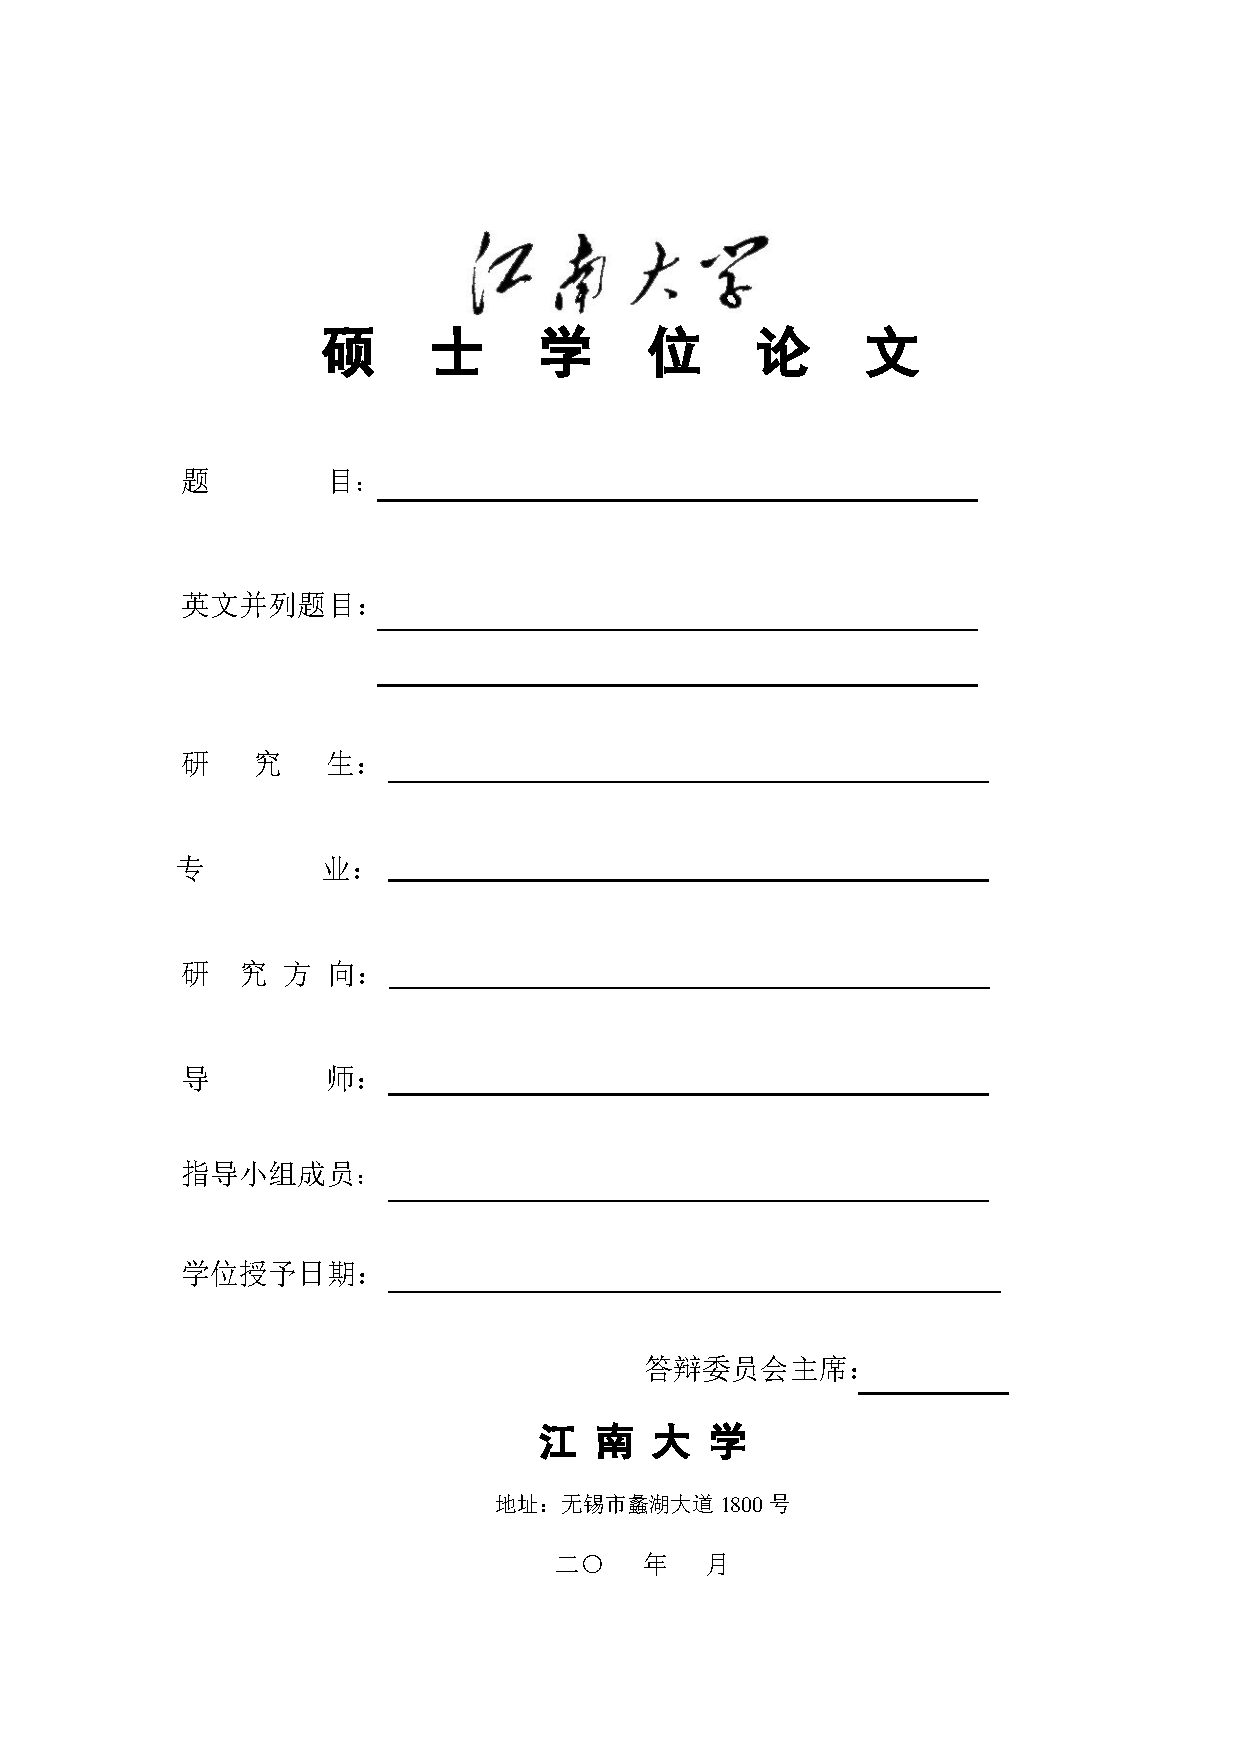
\includepdf{cover.pdf}             % 封面
    \cleardoublepage
    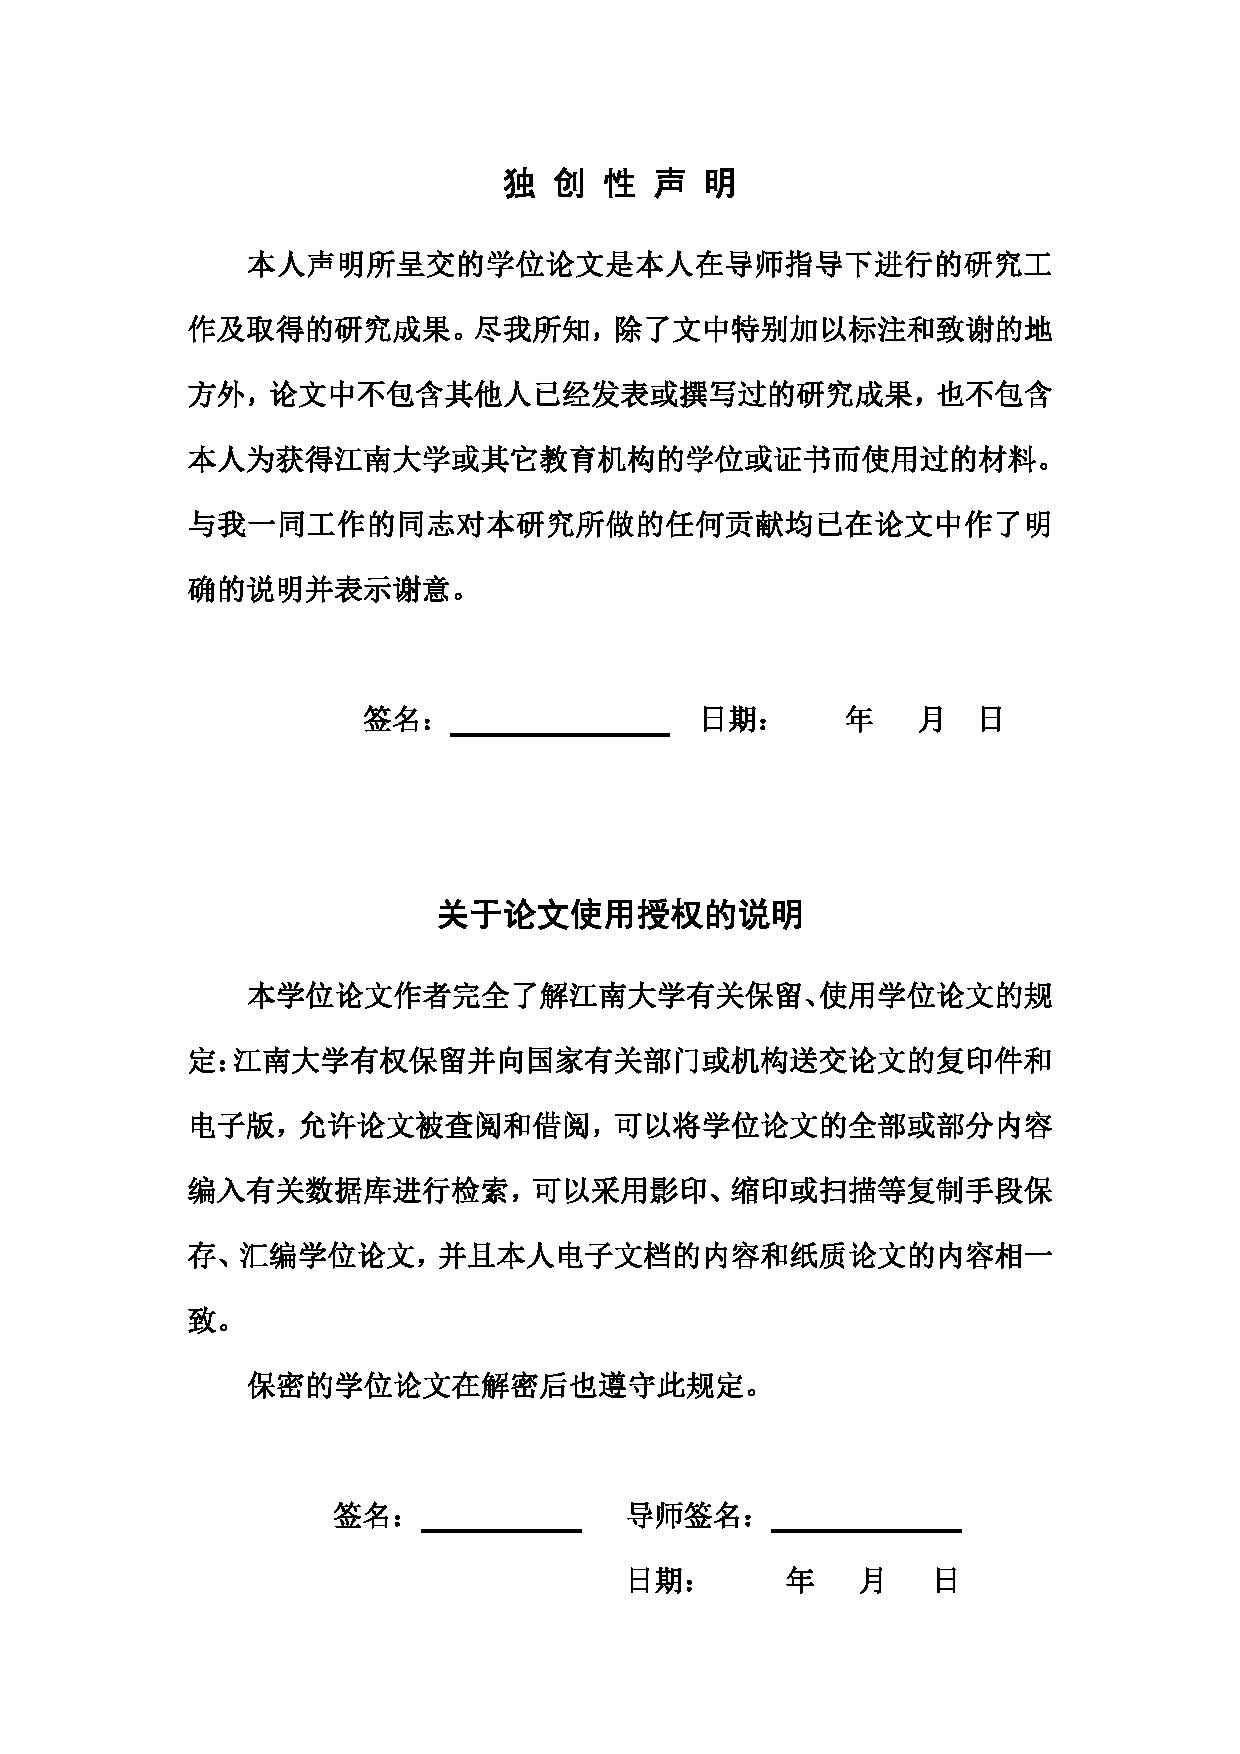
\includepdf{statement.pdf}         % 独创性声明
	\jnfrontmatter                     % 论文开始
	% !Mode:: "TeX:UTF-8"
% !TeX encoding = UTF-8 Unicode
% !TeX program = xelatex
% !TeX root = ../root.tex
%%%%%%%%%%%%%%%%%%%%%%%%%%%%%%%%%%%%%%%%%%%
\jnabstract[zh]   % 以下 中文摘要
%%%%%%%%%%%%%%%%%%%%%%%%%%%%%%%%%%%%%%%%%%%

[[此处填写摘要内容]]


%%%%%%%%%%%%%%%%%%%%%%%%%%%%%%%%%%%%%%%%%%%
%%% 中文关键词(一般3~5个, 以 \sep 隔开)
%%%%%%%%%%%%%%%%%%%%%%%%%%%%%%%%%%%%%%%%%%%

\begin{jnkeywords}
学位论文 \sep 江南大学 \sep 博士 \sep 硕士
\end{jnkeywords}

       % 中文摘要
	% !Mode:: "TeX:UTF-8"
% !TeX encoding = UTF-8 Unicode
% !TeX program = xelatex
% !TeX root = ../root.tex
%%%%%%%%%%%%%%%%%%%%%%%%%%%%%%%%%%%%%%%%%%%
\jnabstract[en]   % 以下 英文摘要
%%%%%%%%%%%%%%%%%%%%%%%%%%%%%%%%%%%%%%%%%%%

[[此处填写英文摘要]]


%%%%%%%%%%%%%%%%%%%%%%%%%%%%%%%%%%%%%%%%%%%
%%% 英文关键词(一般3~5个, 以 \sep 隔开)
%%%%%%%%%%%%%%%%%%%%%%%%%%%%%%%%%%%%%%%%%%%

\begin{jnkeywords}[en]
Thesis \sep Jiangnan University \sep Doctor \sep Master
\end{jnkeywords}
       % 英文摘要
	\jncontents                        % 目录
    \jnmainmatter                      % 正文开始
	% !Mode:: "TeX:UTF-8"
% !TeX encoding = UTF-8 Unicode
% !TeX program = xelatex
% !TeX root = root.tex

% !Mode:: "TeX:UTF-8"
% !TeX encoding = UTF-8 Unicode
% !TeX program = xelatex
% !TeX root = ../root.tex


\chapter{绪论}
\label{ch01}

[[此处填写正文内容]]

% !Mode:: "TeX:UTF-8"
% !TeX encoding = UTF-8 Unicode
% !TeX program = xelatex
% !TeX root = ../root.tex


\chapter{章标题}
\label{ch02}


[[此处填写正文内容]]

% !Mode:: "TeX:UTF-8"
% !TeX encoding = UTF-8 Unicode
% !TeX program = xelatex
% !TeX root = ../root.tex


\chapter{章标题}
\label{ch03}


[[此处填写正文内容]]

% !Mode:: "TeX:UTF-8"
% !TeX encoding = UTF-8 Unicode
% !TeX program = xelatex
% !TeX root = ../root.tex

\providecommand{\emph}[1]{{\kaishu #1}}

\chapter{章标题}
\label{ch04}

[[此处填写正文内容]]

% !Mode:: "TeX:UTF-8"
% !TeX encoding = UTF-8 Unicode
% !TeX program = xelatex
% !TeX root = ../root.tex


\chapter{章标题}
\label{ch05}

[[此处填写正文内容]]

% !Mode:: "TeX:UTF-8"
% !TeX encoding = UTF-8 Unicode
% !TeX program = xelatex
% !TeX root = ../root.tex


\chapter{章标题}
\label{ch06}

[[此处填写正文内容]]


% !Mode:: "TeX:UTF-8"
% !TeX encoding = UTF-8 Unicode
% !TeX program = xelatex
% !TeX root = ../root.tex


\chapter{结论与展望}
\label{ch07}

[[此处填写正文内容]]

% !Mode:: "TeX:UTF-8"
% !TeX encoding = UTF-8 Unicode
% !TeX program = xelatex
% !TeX root = ../root.tex


\chapter{论文模板使用说明}
\label{ch99}


\section{模板介绍}

为了方便撰写江南大学学位论文, 设计本 \LaTeX 模板.
本模板采用 MIT 协议授权, 如有不完善之处, 请自行修改代码.

\subsubsection*{主要内容}

本模板主要包括两个文件:

\begin{tabular}{ll}
\hline
文件 & 说明\\
\hline
{\tt{jnthesis.cls}} & 提供文档类 {\tt{jnthesis}}, 包含论文各部分的格式设置\\
{\tt{jn.bst}} & 提供参考文献格式\\
\hline
\end{tabular}

\subsubsection*{文档类 {\tt{jnthesis.cls}}}

文档类 {\tt jnthesis} 基于 {\tt ctex} 宏包提供的 {\tt ctexbook} 文档类,
依据江南大学学位论文格式(2012版)进行排版,
定义了字体, 字号, 行距, 标题, 页眉, 页脚, 目录, 摘要, 正文等各种格式.
基本用法如下:

\begin{lstlisting}[basicstyle=\ttfamily, frame=single]
\documentclass{jnthesis}
\end{lstlisting}

上述文档默认为博士学位论文, 可以通过设置参数 {\tt doctor} 或 {\tt master} 指定为博士或硕士学位论文, 还可以指定参数 {\tt nodegree} 表示毕业论文而非学位论文,
用法如下:
\begin{lstlisting}[basicstyle=\ttfamily, frame=single]
\documentclass[doctor]{jnthesis} % 博士学位论文
\documentclass[master]{jnthesis} % 硕士学位论文
\documentclass[doctor, nodegree]{jnthesis} % 博士毕业论文
\end{lstlisting}

文档类 {\tt jnthesis} 针对论文结构, 提供了相应的命令.

\begin{lstlisting}[basicstyle=\ttfamily, frame=single]
    \jnfrontmatter                     % 论文开始
    \jnabstract[zh]                    % 中文摘要
    \begin{jnkeywords}
      学位论文 \sep 江南大学 \sep 博士 \sep 硕士
    \end{jnkeywords}
    \jnabstract[en]                    % 英文摘要
    \begin{jnkeywords}[en]
      Thesis \sep Jiangnan University \sep Doctor \sep Master
    \end{jnkeywords}
    \jncontents                        % 目录
    \jnmainmatter                      % 正文开始
    \jnacknowledgements                % 致谢
    \jnreferences                      % 参考文献
    \jnpublications                    % 发表论文列表
\end{lstlisting}

文档类 {\tt jnthesis} 还定义了以下命令:

\begin{lstlisting}[basicstyle=\ttfamily, frame=single]
    \sep                    % 关键词之间的分隔符
    \setbstfile{jn}         % 设置 bst 文件
    \setbibfiles{ref1,ref2} % 指定 bib 文献数据库
    \citeit{refkey}         % 在正文中引用参考文献
\end{lstlisting}

文档类 {\tt jnthesis} 还定义了定理环境:

\begin{lstlisting}[basicstyle=\ttfamily, frame=single]
\begin{theorem}定理\end{theorem}
\end{lstlisting}

类似的还有 {\tt lemma} 引理,
{\tt proposition} 命题,
{\tt assumption} 假设,
{\tt corollary} 推论,
{\tt property} 性质,
{\tt axiom} 公理,
{\tt definition} 定义,
{\tt example} 例,
{\tt remark} 注.


文档类 {\tt jnthesis} 导入了下列宏包,
其具体用法请查阅相关文档.

\begin{tabular}{lll}
\hline
功能 & 宏包 & 参数\\
\hline
标题, 目录 & titlesec, titletoc &\\
页眉页脚 & fancyhdr &\\
字体, 行距 & fontspec, xunicode, setspace &\\
列表 & enumerate, enumitem\\
表格 & booktabs, longtable, &\\
& hhline, threeparttable & \\
参考文献 & natbib & square, super, comma, sort\&compress\\
\hline
数学公式 & amsmath & \\
数学字体 & amsfonts, mathrsfs, mathtools & \\
定理环境 & ntheorem & hyperref, thmmarks, amsmath\\
算法, 代码 & algorithmicx, algpseudocode, listings & \\
\hline
插图, 子图 & graphicx, subfig &\\
双语标题 & bicaption &\\
颜色, 超链接 & color, hyperref &\\
\hline
\end{tabular}


\subsubsection*{参考文献格式 {\tt{jn.bst}}}

参考文献格式 {\tt jn} 可以配合 BibTeX 文献数据库 (.bib) 实现参考文献格式化.

\begin{lstlisting}[basicstyle=\ttfamily, frame=single]
\bibliographystyle{jn}  % 指定参考文献格式
\end{lstlisting}

参考文献具体格式参见文后的参考文献部分\cite{Dupont1974,Aho1986,Chen1990,张全福1991,高景德1987,余勇1998,霍夫斯基1981,张竹生1983,竺可桢1973}.

采用 {\tt natbib} 格式化参考文献的引用.
比如可以用 {\tt cite} 命令引用参考文献,
如\cite{Dupont1974,Aho1986,Chen1990,竺可桢1973},
同时定义了命令 {\tt citeit} 用于在文章内容中引用具体文献,
如文献\citeit{Dupont1974,Aho1986,Chen1990,竺可桢1973}.

对于专业用户, 如果个别类型的文献格式不符合要求, 请修改格式文件 {\tt jn.bst}.

对于一般用户, 如果个别类型的文献格式不符合要求, 请直接修改编译生成的 {\tt root.bbl} 文件.

\subparagraph{注意:} 为生成参考文献, 需执行 {\tt BibTeX} 命令. 该命令生成并重写 {\tt root.bbl} 文件.

\subparagraph{编写 {\tt .bib} 文献数据库常见的问题:}
(1) 建议利用相关软件编写 BibTeX 文献数据库, 如 JabRef.
(2) 标题中个别字母大写时, 用大括号括起来, 如 {\tt title=\{Boundary control of \{PDEs\}\}}. (3) 注意英文人名的正确写法, 如张三的英文名正确写法是 {\tt San Zhang} 或 {\tt S. Zhang} 或 {\tt Zhang, San} 或 {\tt Zhang, S.} 均可.

\section{模板用法}

\subsection{基本用法}

为便于编辑, 通常将长文档分成若干文件.
这里提供了一个具体的模板,
除了以上所说的 {\tt jnthesis.cls} 和 {\tt jn.bst} 两个文件之外,
还包括以下文件:

\begin{tabular}{ll}
\hline
文件 & 说明\\
\hline
{\tt root.tex} & 主文档, 整个文档结构, 用 XeLaTeX 编译此文档\\
{\tt main.tex} & 主要内容, 包含主要章节内容\\
\hline
{\tt cover.doc} & 封面, DOC 文件, 修改编辑后另存为 PDF\\
{\tt cover.pdf} & 封面, PDF 文件, 插入文档\\
{\tt statement.doc} & 声明和授权, DOC 文件, 修改编辑后另存为 PDF\\
{\tt statement.pdf} & 声明和授权, PDF 文件, 插入文档\\
\hline
{\tt setup/settings.tex} & 用户设置, 如: 标题, 作者, 其他宏包和样式等\\
{\tt setup/userdefs.tex} & 用户自定义符号\\
\hline
{\tt preface/e\_abstract.tex} & 英文摘要和英文关键词\\
{\tt preface/c\_abstract.tex} & 中文摘要和中文关键词\\
\hline
{\tt body/ch01.tex} & 第一章内容\\
{\tt body/ch02.tex} & 第二章内容\\
...... & 各章节内容, 不需要的部分可在 {\tt main.tex} 中删除\\
{\tt body/ch99.tex} & 模板使用说明, 不需要时在 {\tt main.tex} 中删除\\
\hline
{\tt appendix/acknowledgements.tex} & 致谢内容\\
{\tt appendix/publications.tex} & 发表论文\\
\hline
{\tt references.bib} & 参考文献数据库\\
{\tt figures/...} & 插图\\
\hline
\end{tabular}


具体用法如下:
\subparagraph{1.} 打开 {\tt root.tex} 文件, 设置文档参数以指定博士(doctor), 硕士(master) 或毕业(nodegree)论文.
\subparagraph{2.} 打开 {\tt main.tex} 文件, 规划论文主要章节. 不需要的章节可以删除或注释掉.
\subparagraph{3.} 修改 {\tt cover.doc} 文件生成封面 {\tt cover.pdf}.
\subparagraph{4.} 修改(如有必要) {\tt statement.doc} 生成 {\tt statement.pdf}.
\subparagraph{5.} 修改 {\tt setup/settings.tex} 设置标题, 作者, 包含其他宏包等其他设置.
\subparagraph{6.} 修改(如有必要) {\tt setup/userdefs.tex} 添加用户自定义符号或命令.
\subparagraph{7.} 修改 {\tt preface/e\_abstract.tex} 添加英文摘要和英文关键词.
\subparagraph{8.} 修改 {\tt preface/c\_abstract.tex} 添加中文摘要和中文关键词.
\subparagraph{9.} 修改 {\tt body/ch01.tex} 等, 撰写各章内容.
\subparagraph{10.} 修改 {\tt appendix/acknowledgements.tex} 添加致谢内容.
\subparagraph{11.} 修改 {\tt appendix/publications.tex} 添加发表论文.
\subparagraph{12.} 修改任何内容后, 用 XeLaTeX 编译 {\tt root.tex} 文件得到最终论文 {\tt root.pdf}. 若参考文献不正确, 首先执行 BibTeX, 再多次(三次以上)执行 XeLaTeX, 直到得到正确的参考文献.

一次完整的编译过程为 XeLaTeX > BibTeX > XeLaTeX > XeLaTeX > XeLaTeX. 通常在引用参考文献没有发生变化时, 仅需要执行一次 XeLaTeX.
由于已经把整个文档划分成多个文件, 加快了编译速度.
当 {\tt bib} 文献数据库或文献引用发生变化时, 为确保最终内容正确, 可以执行一遍完整的编译过程.
引用\cite{高景德1987, 霍夫斯基1981, 余勇1998, 张全福1991, 张竹生1983, 竺可桢1973, Aho1986, Chen1990, Dupont1974}
\subsection{插图}

\subsubsection{设置插图文件路径}

为方便管理, 建议设置插图文件路径.
例如, 若将插图文件全部存放在 {\tt figures} 文件夹下,
可以设置如下:

\begin{lstlisting}[basicstyle=\ttfamily, frame=single]
\graphicspath{{figures/}} % 插图文件路径 (以 / 结尾)
\end{lstlisting}

此后, 使用 {\tt includegraphics} 命令时, 将在指定的文件夹中搜索.
例如, 为了插入图形文件 {\tt figures/logo/logo-lg.jpg},
可以使用以下命令:

\begin{lstlisting}[basicstyle=\ttfamily, frame=single]
\begin{figure}
  \centering
  
\includegraphics{logo/logo-lg.jpg}
  \bicaption{插图例子}{Example of figure}
\end{figure}
\end{lstlisting}

注意其中插图文件名中, 省略了指定的插图路径 {\tt figures/}.
{\tt bicaption} 命令展示了双语标题的用法.
简单标题直接使用 {\tt caption} 命令.
插图效果如图 \ref{fig1} 所示.

\begin{figure}
  \centering
  
\includegraphics{logo/logo-lg.jpg}
  \bicaption{插图例子}{Example of figure}
  \label{fig1}
\end{figure}

\subsubsection{子图}

使用 {\tt subfloat} 命令插入子图(如图 \ref{fig2}).

\begin{lstlisting}[basicstyle=\ttfamily, frame=single]
\begin{figure}
    \centering
    \subfloat[][子图1]{
        
\includegraphics{logo/logo-lg.jpg}}
    \hspace{2em}
    \subfloat[][子图2]{
        
\includegraphics{logo/logo-lg.jpg}}
    \caption{子图的例子}
    \label{fig2}
\end{figure}
\end{lstlisting}

\begin{figure}
    \centering
    \subfloat[][子图1]{
        
\includegraphics{logo/logo-lg.jpg}}
    \hspace{2em}
    \subfloat[][子图2]{
        
\includegraphics{logo/logo-lg.jpg}}
    \caption{子图的例子}
    \label{fig2}
\end{figure}

 % 模板使用说明, 不需要时删除即可
                       % 正文
	% !Mode:: "TeX:UTF-8"
% !TeX encoding = utf-8
% !TeX program = xelatex
% !TeX root = ../root.tex
%%%%%%%%%%%%%%%%%%%%%%%%%%%%%%%%%%%%%%%%%%%
\jnacknowledgements % 以下 致谢部分
%%%%%%%%%%%%%%%%%%%%%%%%%%%%%%%%%%%%%%%%%%%

% 致谢
	\jnreferences                      % 参考文献
	% !Mode:: "TeX:UTF-8"
% !TeX encoding = utf-8
% !TeX program = xelatex
% !TeX root = ../root.tex
%%%%%%%%%%%%%%%%%%%%%%%%%%%%%%%%%%%%%%%%%%%
\jnpublications % 以下 附录: 发表论文列表
%%%%%%%%%%%%%%%%%%%%%%%%%%%%%%%%%%%%%%%%%%%

    % 发表论文列表
\end{document}
